\documentclass[12pt,a4paper,notitlepage,oneside,amsmath,amssymb]{article}
\usepackage{geometry}  % See geometry.pdf to learn the layout options. There are lots.
\geometry{a4paper, margin=1in, noheadfoot} % ... or a4paper or a5paper or ...
\usepackage[utf8]{inputenc}
\usepackage{graphicx}
\graphicspath{{./img/}}
\usepackage{amsmath}
\usepackage{amssymb}
% \usepackage{fontspec}
% \setromanfont{LiHei Pro}
% \XeTeXlinebreaklocale "zh"
% \XeTeXlinebreakskip = 0pt plus 1pt
\usepackage{CJKutf8}
\usepackage{anyfontsize}
\usepackage{caption}
\usepackage{indentfirst}
\usepackage{titlesec}
\usepackage{enumitem}
\usepackage[normalem]{ulem}
\usepackage[most]{tcolorbox}
% \tcbuselibrary{breakable}
% \usepackage{cancel}
\usepackage{xcolor}
% \usepackage[pages=all]{background}
\definecolor{text}{rgb}{0.1, 0.1, 0.1}
\color{black}

\titleformat*{\section}{\large\bfseries}
\titleformat*{\subsection}{\large\bfseries}
\titleformat*{\subsubsection}{\large\bfseries}
\titleformat*{\paragraph}{\large\bfseries}
\titleformat*{\subparagraph}{\large\bfseries}
% \titlespacing*{<command>}{<left>}{<before-sep>}{<after-sep>}
\titlespacing*{\section}{0pt}{15pt}{4pt}


% \setlength{\parindent}{0em}
% \setlength{\parskip}{0.5em}
% \setlength{\columnsep}{0.5cm}
\renewcommand{\baselinestretch}{1.2} % scales the default interline space to 1.5 its default value.

% \setlist[itemize]{topsep=2pt, itemsep=0.2ex, partopsep=0ex, parsep=0ex, nosep, leftmargin=3ex,
% labelindent=1ex, labelwidth=1ex}
% \setlist[enumerate]{topsep=2pt, itemsep=0.2ex, partopsep=0.5ex, parsep=0.2ex, nosep,
%     labelindent=2ex, labelwidth=2ex}

\begin{document}
\begin{CJK*}{UTF8}{bkai}

	\CJKtilde{}
	\CJKindent{}
	\title{\vspace{-10ex}DIP HW2 Report}
	\author{R07922036~邱能賢}
	\date{\vspace{-1ex}\today}

	\maketitle

	\vspace{-5ex}

  \section*{Problem 1: Edge Detection}

	\begin{enumerate}[label=(\alph*)]
		\item Perform first order edge detection as image \(E_1\).

    To perform first order edge detection, I used Roberts cross differentiation and only kept its magnitude.

    The threshold is calculated by first calculate the CDF and set the threshold at the intensity at \(80\%\) of pixels.

		\item Perform second order edge detection as image \(E_2\).

    To perform second order edge detection, I first convolute the image with a low-pass filter then with a separable 8-neighbor laplacian filter.

    \[
            Gaussian =
            \frac{1}{16}
            \begin{bmatrix}
				      1 & 2 & 1 \\
				      2 & 4 & 2 \\
				      1 & 2 & 1
            \end{bmatrix},
            H =
            \frac{1}{8}
			      \begin{bmatrix}
				      -2 & 1 & -2 \\
				      1 & 4  & 1 \\
				      -2 & 1 & -2
            \end{bmatrix}
          \]

    Then, with a threshold of \(\pm 2.5\), set the value to \(\pm 1\) if above the threshold, otherwise \(0\). At last, check zero-crossing considering the 8-neighbor (four directions).

		\item Perform Canny edge detection as image \(E_2\).

    Canny edge detection is done as the following method:

    \begin{enumerate}
      \item Noise reduction with Gaussian filter:

      \[
        Gaussian =
            \frac{1}{159}
            \begin{bmatrix}
				      2 & 4 & 5 & 4 & 2 \\
				      4 & 9 & 12 & 9 & 4 \\
              5 & 12 & 15 & 12 & 5 \\
				      4 & 9 & 12 & 9 & 4 \\
              2 & 4 & 5 & 4 & 2
            \end{bmatrix}
            \]

      \item Compute gradient magnitude and orientation with Sobel filter:

      \[
        G_x =
			      \begin{bmatrix}
				      -1 & 0 & 1 \\
				      -2 & 0 & 2 \\
				      -1 & 0 & 1
            \end{bmatrix},
            G_y =
			      \begin{bmatrix}
				      -1 & -2 & -1 \\
				      0 & 0 & 0 \\
				      1 & 2 & 1
            \end{bmatrix}
            \]

      \item Non-maximal suppression:

      The orientation is modded to \([0, \pi / 128 ]\) and the nearest neighbor is calculate by interpolation of the 8-neighbor.

      \item Hysteretic thresholding:

      The higher threshold is set to the intensity at \(90\%\) of CDF, and the lower threshold is the half of the higher value.

      \item Connected component labeling method:

      Using breadth-first search considering all the 8-neighbor.

    \end{enumerate}

    \begin{table}
    \begin{tabular}[h!]{ccccc}
      Original & Gradient & Suppression & Thresholding & Result \\
      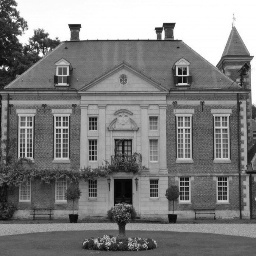
\includegraphics[width=.18\linewidth]{sample1}&
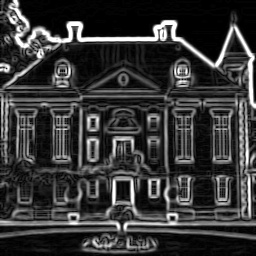
\includegraphics[width=.18\linewidth]{E3_sample1_gradient}&
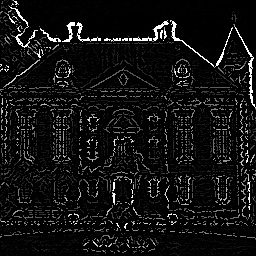
\includegraphics[width=.18\linewidth]{E3_sample1_suppression}&
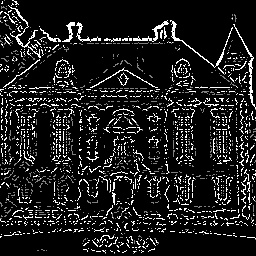
\includegraphics[width=.18\linewidth]{E3_sample1_thresholding}&
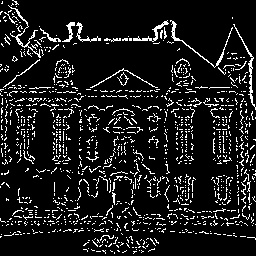
\includegraphics[width=.18\linewidth]{E3_sample1}\\
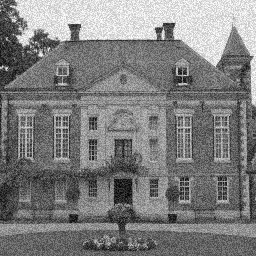
\includegraphics[width=.18\linewidth]{sample2}&
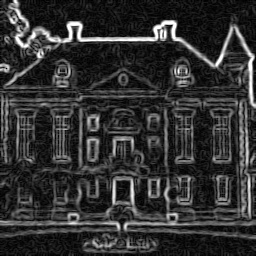
\includegraphics[width=.18\linewidth]{E3_sample2_gradient}&
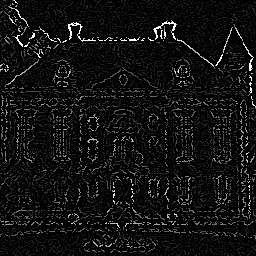
\includegraphics[width=.18\linewidth]{E3_sample2_suppression}&
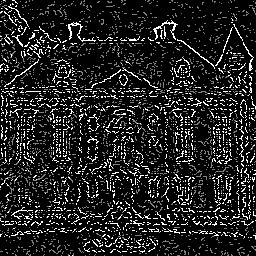
\includegraphics[width=.18\linewidth]{E3_sample2_thresholding}&

\includegraphics[width=.18\linewidth]{E3_sample2}\\
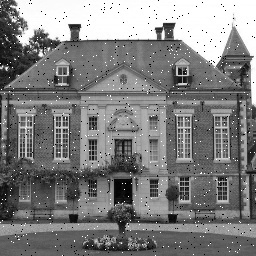
\includegraphics[width=.18\linewidth]{sample3}&
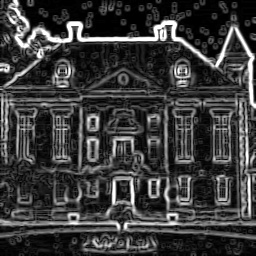
\includegraphics[width=.18\linewidth]{E3_sample3_gradient}&
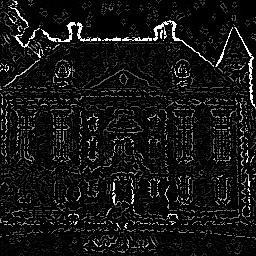
\includegraphics[width=.18\linewidth]{E3_sample3_suppression}&
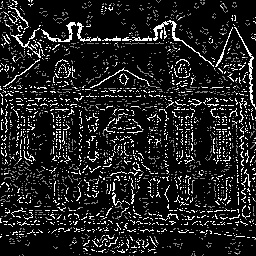
\includegraphics[width=.18\linewidth]{E3_sample3_thresholding}&
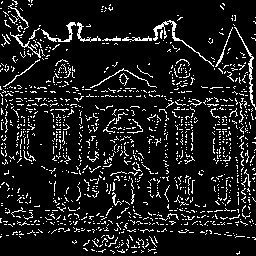
\includegraphics[width=.18\linewidth]{E3_sample3}\\
\end{tabular}
\caption{Result after each step of Canny edge detection.}
\end{table}

		      \begin{table}
		      \begin{tabular}[h!]{cccc}
			                                                        & sample1.raw & sample2.raw & sample3.raw \\
			      original                                          &
			      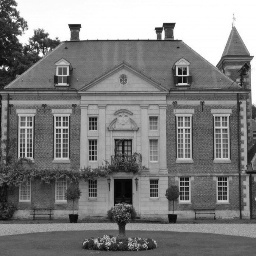
\includegraphics[width=.25\linewidth]{sample1}    &
			      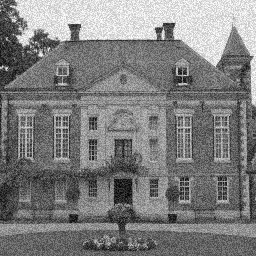
\includegraphics[width=.25\linewidth]{sample2}    &
			      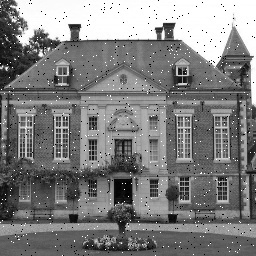
\includegraphics[width=.25\linewidth]{sample3}                                              \\
			      \(E_1\)                                           &
			      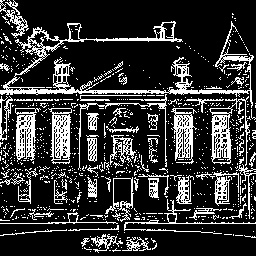
\includegraphics[width=.25\linewidth]{E1_sample1} &
			      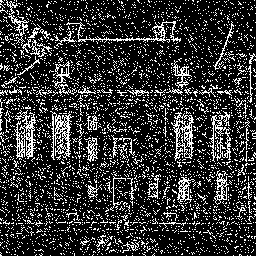
\includegraphics[width=.25\linewidth]{E1_sample2} &
			      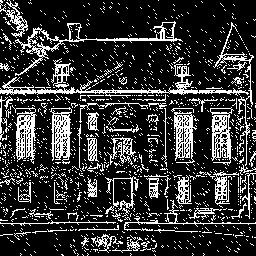
\includegraphics[width=.25\linewidth]{E1_sample3}                                           \\
			      \(E_2\)                                           &
			      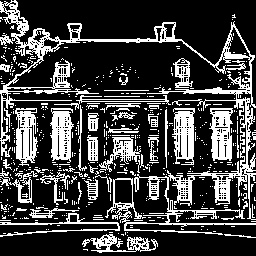
\includegraphics[width=.25\linewidth]{E2_sample1} &
			      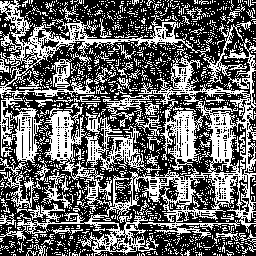
\includegraphics[width=.25\linewidth]{E2_sample2} &
			      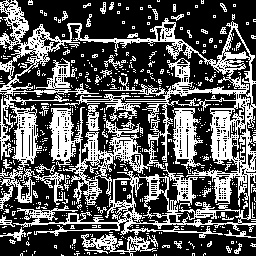
\includegraphics[width=.25\linewidth]{E2_sample3}                                           \\
			      \(E_3\)                                           &
			      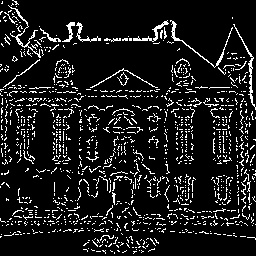
\includegraphics[width=.25\linewidth]{E3_sample1} &
			      
\includegraphics[width=.25\linewidth]{E3_sample2} &
			      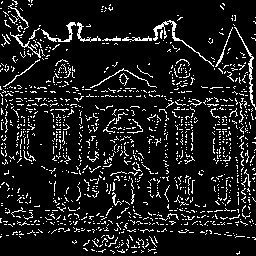
\includegraphics[width=.25\linewidth]{E3_sample3}                                           \\
          \end{tabular}
          \caption{Result of different edge detecting method.}
        \end{table}
  \end{enumerate}

  \newpage

	\section*{Problem 2: Noise Removal}
	\begin{enumerate}[label=(\alph*)]
		\item Perform edge crispening on \(I_2\) as image \(C\).

		      To perform edge crispening, I simple convolute the image with the following high pass filter, which showed the best result in the textbook:
		      \[
			      H =
			      \begin{bmatrix}
				      -1 & -1 & -1 \\
				      -1 & 9  & -1 \\
				      -1 & -1 & -1
			      \end{bmatrix}
		      \]

		      As a result, I think not only the edge is crispened, but also the contrast is increased.

		      \begin{figure}[hbt!]
			      \centering
			      \begin{minipage}{.4\textwidth}
				      \centering
				      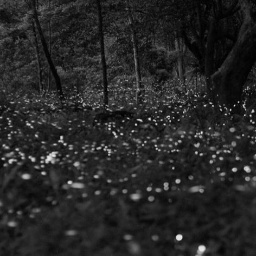
\includegraphics[width=.8\linewidth]{sample4}
				      \caption*{\(I_2\), sample4.raw}
			      \end{minipage}%
			      \begin{minipage}{.4\textwidth}
				      \centering
				      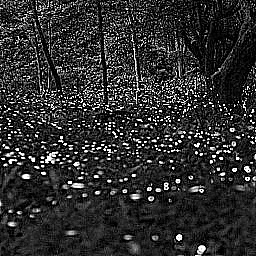
\includegraphics[width=.8\linewidth]{image_C}
				      \caption*{image \(C\)}
			      \end{minipage}
		      \end{figure}

		\item Design a warping method to produce \(D\) from \(C\). \(D\) is a swirled disk with diameter of 256 pixels.

    For coordinate \((i,j)\) relative to the center of the image:
    \begin{enumerate}
      \item Wrap to a circle:
      \[r = \sqrt{i^2 + j^2}, \theta = atan (\frac{j}{i})\]

      \[(r,\theta ) \rightarrow (r \times \max (|\cos(\theta)|, |\sin(\theta)|), \theta)\]

      \item Swirl transformation, \(\rho\) is the radius of the image:

      \[(r,\theta ) \rightarrow (r , (\mathrm{swirl\ angle}) \times (1-\frac{r}{\rho}) \theta), \rho = 128\]
    \end{enumerate}

		      \begin{tabular}[h!]{cccc}
			      Image \(C\)                                           & Wrap to a disk & Swirl \( \pi/4 \) & Swirl \( \pi/2 \) \\
			      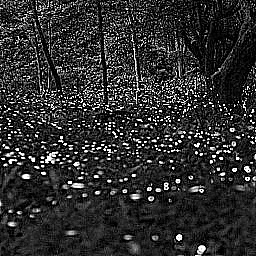
\includegraphics[width=.23\linewidth]{image_C}        &
			      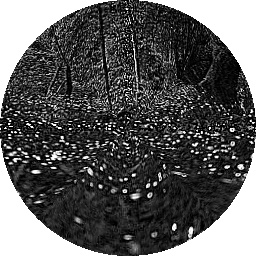
\includegraphics[width=.23\linewidth]{image_D_round}  &
			      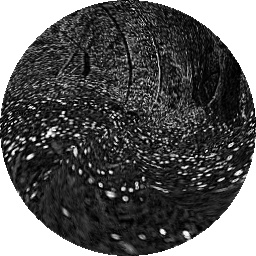
\includegraphics[width=.23\linewidth]{image_D_0_25PI} &
			      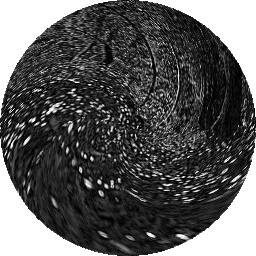
\includegraphics[width=.23\linewidth]{image_D_0_5PI}                                                           \\
		      \end{tabular}

	\end{enumerate}

	\clearpage

\end{CJK*}
\end{document}
